    \documentclass[tikz, border=20pt]{standalone}
    \usetikzlibrary{shapes.geometric, arrows.meta, positioning, shadows, fit, backgrounds, calc}

    \begin{document}
    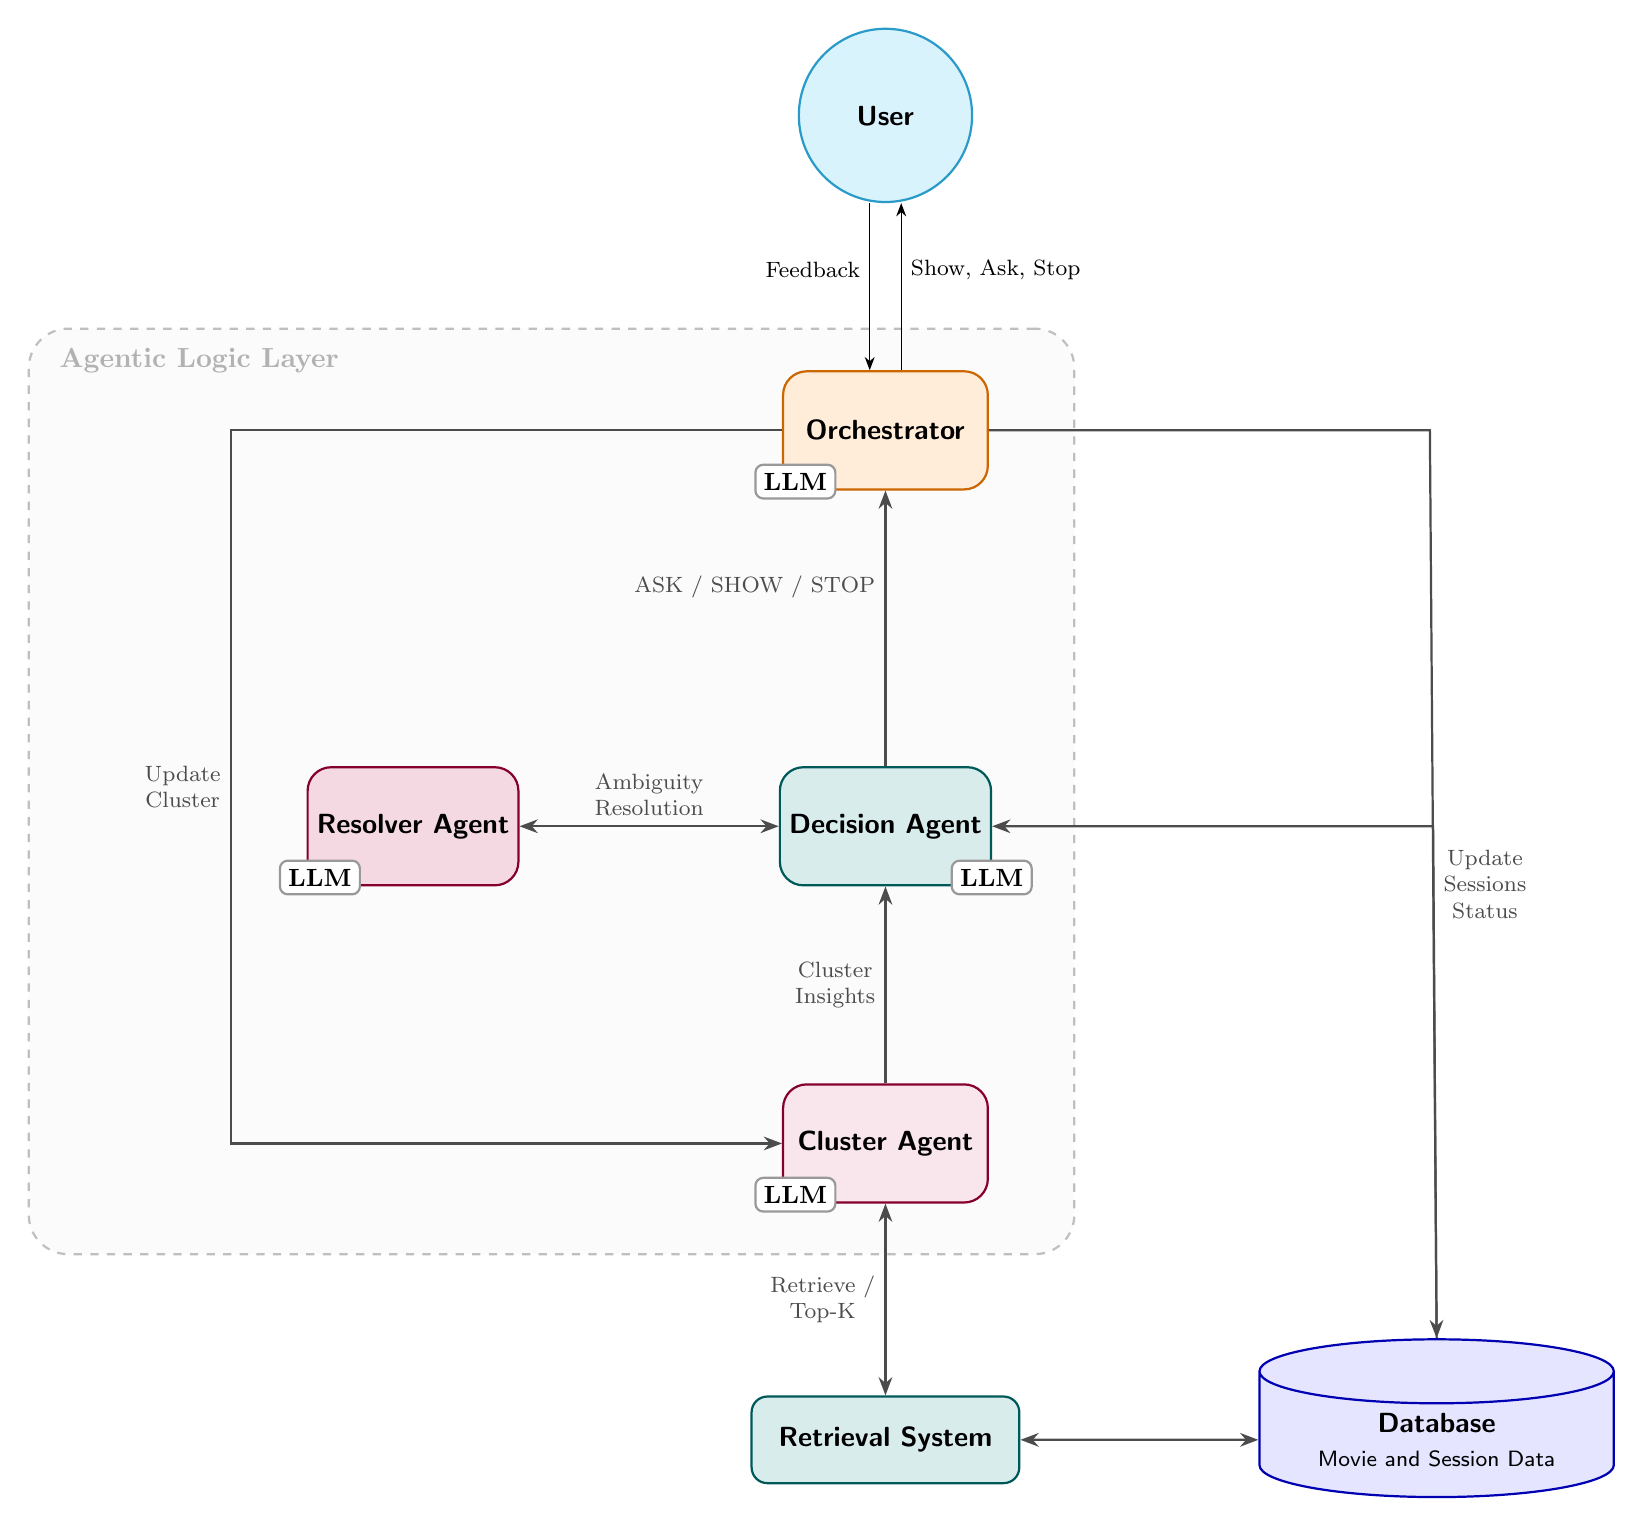
\begin{tikzpicture}[
        font=\sffamily,
        >=Stealth,
        node distance=1.5cm and 2.5cm,
        every node/.style={align=center},
        user/.style={circle, draw=cyan!80!black, fill=cyan!15, thick, minimum size=2.2cm},
        oracle/.style={circle, draw=red!80!black, fill=red!15, thick, minimum size=2.2cm},
        db/.style={cylinder, shape border rotate=90, draw=blue!70!black, fill=blue!10, thick, aspect=0.25, minimum width=4.5cm, minimum height=1.8cm},
        judge/.style={rectangle, draw=red!80!black, fill=red!10, thick, rounded corners=3mm, minimum width=4cm, minimum height=1.3cm},
        cluster/.style={rectangle, draw=purple!70!black, fill=purple!10, thick, rounded corners=3mm, minimum width=2.6cm, minimum height=1.5cm},
        resolver/.style={rectangle, draw=purple!70!black, fill=purple!15, thick, rounded corners=3mm, minimum width=2.6cm, minimum height=1.5cm},
        orchestrator/.style={rectangle, draw=orange!80!black, fill=orange!15, thick, rounded corners=3mm, minimum width=2.6cm, minimum height=1.5cm},
        output_agent/.style={rectangle, draw=green!60!black, fill=green!15, thick, rounded corners=3mm, minimum width=2.6cm, minimum height=1.5cm},
        decision/.style={rectangle, draw=teal!70!black, fill=teal!15, thick, rounded corners=3mm, minimum width=2.6cm, minimum height=1.5cm},
        retrieval/.style={rectangle, draw=teal!70!black, fill=teal!15, thick, rounded corners=2mm, minimum width=3.4cm, minimum height=1.1cm},
        llm_node/.style={draw=gray!80, fill=white, thick, inner sep=3pt, font=\bfseries\small, rounded corners=1mm},
        arrow/.style={->, thick, color=black!70},
        biarrow/.style={<->, thick, color=black!70},
        judge_arrow/.style={->, dashed, thick, color=red!60!black}
    ]

    % ==================== orchestrator ====================
    \node[orchestrator] (orchestrator) {\textbf{Orchestrator}};
    \node[llm_node, anchor=south west] (llm2) at ([xshift=-10pt, yshift=-25pt]orchestrator.west) {LLM};<s

    % ==================== ORACLE (upper) ====================
    \node[user] (user) at ([xshift=0pt, yshift=4cm]orchestrator) {\textbf{User}};

    % ==================== MIDDLE AGENT LAYER ====================
    \node[resolver, below=3.5cm of orchestrator, xshift=-6cm] (resolver) {\textbf{Resolver Agent}};
    \node[decision,    below=3.5cm of orchestrator, xshift=0cm]  (decision)      {\textbf{Decision Agent}};
    \node[llm_node, anchor=south west] (llm1) at ([xshift=-10pt, yshift=-25pt]resolver.west) {LLM};
    \node[llm_node, anchor=south west] (llm3) at ([xshift=-15pt, yshift=-25pt]decision.east)      {LLM};

    % ==================== cluster LAYER ====================
    \node[cluster, below=2.5cm of decision] (cluster) {\textbf{Cluster Agent}};
    \node[llm_node, anchor=south west] (llm4) at ([xshift=-10pt, yshift=-25pt]cluster.west) {LLM};


    % ==================== KNOWLEDGE BASE (same horizontal level) ====================
    \node[retrieval] (retrieval) at ([xshift=0cm, yshift=-3cm]cluster.south) {\textbf{Retrieval System}};
    \node[db] (db) at ([xshift=7cm,  yshift=-3cm]cluster.south) {\textbf{Database}\\\footnotesize Movie and Session Data};
    \coordinate (agentsWestPad) at ([xshift=-3cm]resolver.west);

    % ==================== AGENTIC LAYER BACKGROUND ====================
    \begin{scope}[on background layer]
        \node[fill=gray!3, rounded corners=5mm, draw=gray!50, dashed, thick,
            fit=(agentsWestPad)(resolver)(decision)(cluster)(orchestrator)(llm1)(llm2)(llm3)(llm4),
            inner sep=15pt] (agents) {};
        \node[anchor=north west, font=\bfseries, color=gray!60]
            at ([xshift=8pt,yshift=-4pt]agents.north west) {Agentic Logic Layer};
    \end{scope}

    % ==================== CONNECTIONS ====================

    % ---- User <-> orchestrator (two separate arrows) ----
    \draw[->] ([xshift=-0.20cm]user.south) -|
        ([xshift=-0.20cm]orchestrator.north)
        node[left, pos=0.7, font=\footnotesize] {Feedback};

    \draw[->] ([xshift=0.20cm]orchestrator.north) -|
        ([xshift=0.20cm]user.south)
        node[right, pos=0.8, font=\footnotesize] {Show, Ask, Stop};


    % ---- orchestrator down to Middle Agents ----
    \coordinate (orchestratorDown1) at ([xshift=-4cm, yshift=-1.75cm]orchestrator.south);
    \coordinate (orchestratorDown3) at ([xshift= 4cm, yshift=-1.75cm]orchestrator.south);

    % ---- Decision Agent to Orchestrator (feedback loop) ----
    \draw[arrow] (decision.north) |-
        (orchestratorDown3 -| decision.north) --
        node[left, pos=0.3, font=\footnotesize] {ASK / SHOW / STOP}
        (orchestrator.south);

    % ---- Resolver Agent <-> Decision Agent (horizontal, same level) ----
    \draw[biarrow] (resolver.east) --
        node[above, pos=0.5, font=\footnotesize] {Ambiguity\\Resolution}
        (decision.west);

    % --- Orchestrator to Cluster Agent ---
    \coordinate (orchestratorLeft) at ([xshift=-7cm, yshift=0]orchestrator.west);
    \coordinate (clusterWest) at ([xshift=-7cm, yshift=0]cluster.west);
    \draw[arrow] ([yshift=0cm]orchestrator.west) -- (orchestratorLeft) --
        node[left, pos=0.5, font=\footnotesize] {Update\\Cluster}
        (clusterWest) -- (cluster.west);

    % --- Cluster Agent to Decision Agent (feedback loop) ---
    \draw[arrow] (cluster.north) --
        node[left, pos=0.5, font=\footnotesize] {Cluster\\Insights}
        (decision.south);

    % ---- cluster <-> Retrieval (left, entering from north) ----
    \draw[biarrow] ([xshift=0cm]cluster.south) --
        node[left, pos=0.5, font=\footnotesize] {Retrieve /\\Top-K}
        (retrieval.north);

    % ---- Retrieval <-> Database (horizontal, same level) ----
    \draw[biarrow] (retrieval.east) -- (db.west);

    % --- Orchestrator to Midpoint (Decision, Orchestrator, Database) ---
    \coordinate (orchestratorRight) at ([xshift=5.6cm, yshift=0cm]orchestrator.east);
    \coordinate (decisionRight) at ([xshift=5.6cm, yshift=0]decision.east);
    \coordinate (dbTop) at ([xshift=0cm, yshift=0cm]db.north);
    \draw[arrow] ([yshift=0cm]orchestrator.east) -- (orchestratorRight) --
        node[right, pos=0.5, font=\footnotesize] {Update\\Sessions\\Status}
        (db.north);

    % --- DB to Decision Agent (feedback loop) ---
    \draw[arrow] (dbTop) -- (decisionRight) -- (decision.east);


    \end{tikzpicture}
    \end{document}
